\documentclass[border=1.5pt]{standalone}
\usepackage{amsmath,amssymb}
\usepackage{tikz}
\usetikzlibrary{arrows.meta,calc,positioning,shapes,shapes.misc,shapes.geometric,backgrounds,fit,decorations.pathreplacing,quantikz2}
% Shared colors and styles for the XYZ^2 figures.
% Pauli types: bright tones for fills and bands, deep (800) shades of the same hues for labels.
% The label shades keep the hue of each Pauli, are well separated from each other (CIEDE2000 > 20)
% and have a contrast ratio of at least 2.9 on the coral cells and 4.5 on the sunflower cells.
\definecolor{PauliX}{HTML}{F97316}
\definecolor{PauliY}{HTML}{EC4899}
\definecolor{PauliZ}{HTML}{9333EA}
\definecolor{PauliXText}{HTML}{AC340B}
\definecolor{PauliYText}{HTML}{9D174D}
\definecolor{PauliZText}{HTML}{5B21B6}
% Generator classes: S0 (class B, even links, coral) and gauge (class A, odd links, sunflower)
\definecolor{Szero}{HTML}{F0435E}
\definecolor{SzeroText}{HTML}{BE123C}
\definecolor{Gauge}{HTML}{F59E0B}
\definecolor{GaugeText}{HTML}{B45309}
\colorlet{GaugeGray}{Gauge}
\definecolor{ClassB}{HTML}{FF8A99}
\definecolor{ClassA}{HTML}{FFD23F}
% Logical operators (X-bar violet, Z-bar crimson), errors, ink
\definecolor{LogicalZ}{HTML}{E11D48}
\definecolor{LogicalGold}{HTML}{7C3AED}
\definecolor{ErrRed}{HTML}{1C1917}
\definecolor{InkDark}{HTML}{292524}
\definecolor{InkSoft}{HTML}{57534E}
% Labels drawn on top of colored cells
\colorlet{CellText}{InkDark}
% Noise channels
\definecolor{ErrFlip}{HTML}{EF4444}
\definecolor{Idle}{HTML}{EC4899}
\definecolor{TwoQ}{HTML}{7C3AED}
% Protocol steps
\definecolor{StepPrep}{HTML}{F97316}
\definecolor{StepMeas}{HTML}{D946EF}
\definecolor{StepDec}{HTML}{7C3AED}
\definecolor{StepRec}{HTML}{DB2777}
\tikzset{
  qb/.style={circle, draw=InkDark, line width=0.6pt, fill=white,
             minimum size=4.2mm, inner sep=0pt, font=\scriptsize},
  qbsmall/.style={circle, draw=InkDark, line width=0.5pt, fill=white,
             minimum size=2.6mm, inner sep=0pt},
  hexedge/.style={line width=0.65pt, draw=InkSoft},
  linkedge/.style={line width=1.6pt, draw=InkDark},
  bndedge/.style={line width=0.65pt, draw=InkSoft, densely dashed},
  plabel/.style={font=\scriptsize\bfseries, inner sep=1pt},
  panel/.style={font=\small\bfseries, anchor=north west},
}

\providecommand{\ket}[1]{\left|#1\right\rangle}

\begin{document}
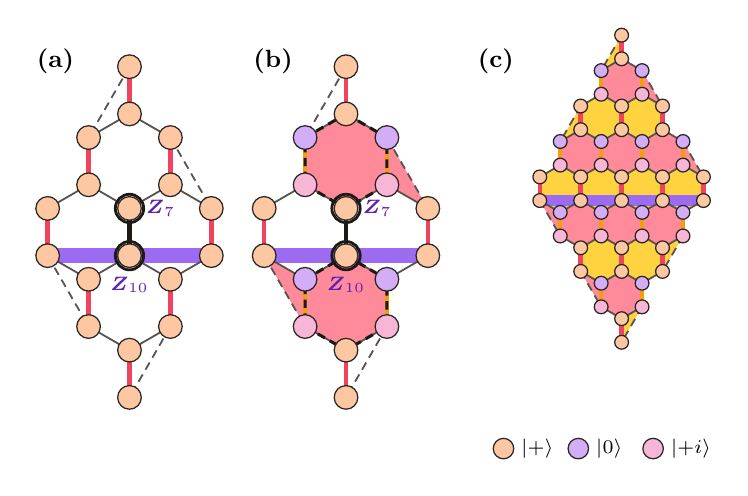
\begin{tikzpicture}
\begin{scope}[shift={(0,0)}, scale=0.6]\fill[white] (0.000,-0.500) -- (0.866,-1.000) -- (0.866,-2.000) -- (0.000,-2.500) -- (-0.866,-2.000) -- (-0.866,-1.000) -- cycle;
\fill[white] (0.866,-2.000) -- (1.732,-2.500) -- (1.732,-3.500) -- (0.866,-4.000) -- (0.000,-3.500) -- (0.000,-2.500) -- cycle;
\fill[white] (-0.866,-2.000) -- (0.000,-2.500) -- (0.000,-3.500) -- (-0.866,-4.000) -- (-1.732,-3.500) -- (-1.732,-2.500) -- cycle;
\fill[white] (0.000,-3.500) -- (0.866,-4.000) -- (0.866,-5.000) -- (0.000,-5.500) -- (-0.866,-5.000) -- (-0.866,-4.000) -- cycle;
\fill[white] (-0.866,-1.000) -- (0.000,-0.500) -- (0.000,0.500) -- cycle;
\fill[white] (-0.866,-5.000) -- (-0.866,-4.000) -- (-1.732,-3.500) -- cycle;
\fill[white] (0.866,-2.000) -- (1.732,-2.500) -- (0.866,-1.000) -- cycle;
\fill[white] (0.000,-6.500) -- (0.866,-5.000) -- (0.000,-5.500) -- cycle;
\draw[line width=5.5pt, draw=LogicalGold!75, line cap=round, line join=round] (-1.732,-3.500) -- (0.000,-3.500) -- (1.732,-3.500);
\draw[hexedge] (0.000,-0.500) -- (-0.866,-1.000);
\draw[hexedge] (0.000,-0.500) -- (0.866,-1.000);
\draw[hexedge] (-0.866,-1.000) -- (-0.866,-2.000);
\draw[hexedge] (0.866,-1.000) -- (0.866,-2.000);
\draw[hexedge] (-0.866,-2.000) -- (-1.732,-2.500);
\draw[hexedge] (-0.866,-2.000) -- (0.000,-2.500);
\draw[hexedge] (0.866,-2.000) -- (0.000,-2.500);
\draw[hexedge] (0.866,-2.000) -- (1.732,-2.500);
\draw[hexedge] (-1.732,-2.500) -- (-1.732,-3.500);
\draw[hexedge] (0.000,-2.500) -- (0.000,-3.500);
\draw[hexedge] (1.732,-2.500) -- (1.732,-3.500);
\draw[hexedge] (-1.732,-3.500) -- (-0.866,-4.000);
\draw[hexedge] (0.000,-3.500) -- (-0.866,-4.000);
\draw[hexedge] (0.000,-3.500) -- (0.866,-4.000);
\draw[hexedge] (1.732,-3.500) -- (0.866,-4.000);
\draw[hexedge] (-0.866,-4.000) -- (-0.866,-5.000);
\draw[hexedge] (0.866,-4.000) -- (0.866,-5.000);
\draw[hexedge] (-0.866,-5.000) -- (0.000,-5.500);
\draw[hexedge] (0.866,-5.000) -- (0.000,-5.500);
\draw[bndedge] (0.000,0.500) -- (-0.866,-1.000);
\draw[bndedge] (-1.732,-3.500) -- (-0.866,-5.000);
\draw[bndedge] (0.866,-1.000) -- (1.732,-2.500);
\draw[bndedge] (0.866,-5.000) -- (0.000,-6.500);
\draw[linkedge, draw=Szero] (0.000,0.500) -- (0.000,-0.500);
\draw[linkedge, draw=Szero] (0.866,-1.000) -- (0.866,-2.000);
\draw[linkedge, draw=Szero] (1.732,-2.500) -- (1.732,-3.500);
\draw[linkedge, draw=Szero] (-0.866,-1.000) -- (-0.866,-2.000);
\draw[linkedge, draw=ErrRed] (0.000,-2.500) -- (0.000,-3.500);
\draw[linkedge, draw=Szero] (0.866,-4.000) -- (0.866,-5.000);
\draw[linkedge, draw=Szero] (-1.732,-2.500) -- (-1.732,-3.500);
\draw[linkedge, draw=Szero] (-0.866,-4.000) -- (-0.866,-5.000);
\draw[linkedge, draw=Szero] (0.000,-5.500) -- (0.000,-6.500);

\node[circle, draw=InkDark, line width=0.45pt, fill=PauliX!40, minimum size=3.0mm, inner sep=0pt] (q0) at (0.000,0.500) {};
\node[circle, draw=InkDark, line width=0.45pt, fill=PauliX!40, minimum size=3.0mm, inner sep=0pt] (q1) at (0.000,-0.500) {};
\node[circle, draw=InkDark, line width=0.45pt, fill=PauliX!40, minimum size=3.0mm, inner sep=0pt] (q2) at (-0.866,-1.000) {};
\node[circle, draw=InkDark, line width=0.45pt, fill=PauliX!40, minimum size=3.0mm, inner sep=0pt] (q3) at (0.866,-1.000) {};
\node[circle, draw=InkDark, line width=0.45pt, fill=PauliX!40, minimum size=3.0mm, inner sep=0pt] (q4) at (-0.866,-2.000) {};
\node[circle, draw=InkDark, line width=0.45pt, fill=PauliX!40, minimum size=3.0mm, inner sep=0pt] (q5) at (0.866,-2.000) {};
\node[circle, draw=InkDark, line width=0.45pt, fill=PauliX!40, minimum size=3.0mm, inner sep=0pt] (q6) at (-1.732,-2.500) {};
\node[circle, draw=InkDark, line width=0.45pt, fill=PauliX!40, minimum size=3.0mm, inner sep=0pt] (q7) at (0.000,-2.500) {};
\node[circle, draw=InkDark, line width=0.45pt, fill=PauliX!40, minimum size=3.0mm, inner sep=0pt] (q8) at (1.732,-2.500) {};
\node[circle, draw=InkDark, line width=0.45pt, fill=PauliX!40, minimum size=3.0mm, inner sep=0pt] (q9) at (-1.732,-3.500) {};
\node[circle, draw=InkDark, line width=0.45pt, fill=PauliX!40, minimum size=3.0mm, inner sep=0pt] (q10) at (0.000,-3.500) {};
\node[circle, draw=InkDark, line width=0.45pt, fill=PauliX!40, minimum size=3.0mm, inner sep=0pt] (q11) at (1.732,-3.500) {};
\node[circle, draw=InkDark, line width=0.45pt, fill=PauliX!40, minimum size=3.0mm, inner sep=0pt] (q12) at (-0.866,-4.000) {};
\node[circle, draw=InkDark, line width=0.45pt, fill=PauliX!40, minimum size=3.0mm, inner sep=0pt] (q13) at (0.866,-4.000) {};
\node[circle, draw=InkDark, line width=0.45pt, fill=PauliX!40, minimum size=3.0mm, inner sep=0pt] (q14) at (-0.866,-5.000) {};
\node[circle, draw=InkDark, line width=0.45pt, fill=PauliX!40, minimum size=3.0mm, inner sep=0pt] (q15) at (0.866,-5.000) {};
\node[circle, draw=InkDark, line width=0.45pt, fill=PauliX!40, minimum size=3.0mm, inner sep=0pt] (q16) at (0.000,-5.500) {};
\node[circle, draw=InkDark, line width=0.45pt, fill=PauliX!40, minimum size=3.0mm, inner sep=0pt] (q17) at (0.000,-6.500) {};
\node[font=\scriptsize, text=PauliZText, inner sep=0.5pt] at ($(q7)+(0:0.66)$) {$\boldsymbol{Z}_7$};
\node[font=\scriptsize, text=PauliZText, inner sep=0.5pt] at ($(q10)+(-90:0.62)$) {$\boldsymbol{Z}_{10}$};
\draw[ErrRed, line width=1.0pt] (q7) circle (0.3);
\draw[ErrRed, line width=1.0pt] (q10) circle (0.3);\end{scope}
\begin{scope}[shift={(2.75,0)}, scale=0.6]\fill[ClassB] (0.000,-0.500) -- (0.866,-1.000) -- (0.866,-2.000) -- (0.000,-2.500) -- (-0.866,-2.000) -- (-0.866,-1.000) -- cycle;
\fill[white] (0.866,-2.000) -- (1.732,-2.500) -- (1.732,-3.500) -- (0.866,-4.000) -- (0.000,-3.500) -- (0.000,-2.500) -- cycle;
\fill[white] (-0.866,-2.000) -- (0.000,-2.500) -- (0.000,-3.500) -- (-0.866,-4.000) -- (-1.732,-3.500) -- (-1.732,-2.500) -- cycle;
\fill[ClassB] (0.000,-3.500) -- (0.866,-4.000) -- (0.866,-5.000) -- (0.000,-5.500) -- (-0.866,-5.000) -- (-0.866,-4.000) -- cycle;
\fill[white] (-0.866,-1.000) -- (0.000,-0.500) -- (0.000,0.500) -- cycle;
\fill[ClassB] (-0.866,-5.000) -- (-0.866,-4.000) -- (-1.732,-3.500) -- cycle;
\fill[ClassB] (0.866,-2.000) -- (1.732,-2.500) -- (0.866,-1.000) -- cycle;
\fill[white] (0.000,-6.500) -- (0.866,-5.000) -- (0.000,-5.500) -- cycle;
\draw[line width=5.5pt, draw=LogicalGold!75, line cap=round, line join=round] (-1.732,-3.500) -- (0.000,-3.500) -- (1.732,-3.500);
\draw[hexedge] (0.000,-0.500) -- (-0.866,-1.000);
\draw[hexedge] (0.000,-0.500) -- (0.866,-1.000);
\draw[hexedge] (-0.866,-1.000) -- (-0.866,-2.000);
\draw[hexedge] (0.866,-1.000) -- (0.866,-2.000);
\draw[hexedge] (-0.866,-2.000) -- (-1.732,-2.500);
\draw[hexedge] (-0.866,-2.000) -- (0.000,-2.500);
\draw[hexedge] (0.866,-2.000) -- (0.000,-2.500);
\draw[hexedge] (0.866,-2.000) -- (1.732,-2.500);
\draw[hexedge] (-1.732,-2.500) -- (-1.732,-3.500);
\draw[hexedge] (0.000,-2.500) -- (0.000,-3.500);
\draw[hexedge] (1.732,-2.500) -- (1.732,-3.500);
\draw[hexedge] (-1.732,-3.500) -- (-0.866,-4.000);
\draw[hexedge] (0.000,-3.500) -- (-0.866,-4.000);
\draw[hexedge] (0.000,-3.500) -- (0.866,-4.000);
\draw[hexedge] (1.732,-3.500) -- (0.866,-4.000);
\draw[hexedge] (-0.866,-4.000) -- (-0.866,-5.000);
\draw[hexedge] (0.866,-4.000) -- (0.866,-5.000);
\draw[hexedge] (-0.866,-5.000) -- (0.000,-5.500);
\draw[hexedge] (0.866,-5.000) -- (0.000,-5.500);
\draw[bndedge] (0.000,0.500) -- (-0.866,-1.000);
\draw[bndedge] (-1.732,-3.500) -- (-0.866,-5.000);
\draw[bndedge] (0.866,-1.000) -- (1.732,-2.500);
\draw[bndedge] (0.866,-5.000) -- (0.000,-6.500);
\draw[linkedge, draw=Szero] (0.000,0.500) -- (0.000,-0.500);
\draw[linkedge, draw=Gauge] (0.866,-1.000) -- (0.866,-2.000);
\draw[linkedge, draw=Szero] (1.732,-2.500) -- (1.732,-3.500);
\draw[linkedge, draw=Gauge] (-0.866,-1.000) -- (-0.866,-2.000);
\draw[linkedge, draw=ErrRed] (0.000,-2.500) -- (0.000,-3.500);
\draw[linkedge, draw=Gauge] (0.866,-4.000) -- (0.866,-5.000);
\draw[linkedge, draw=Szero] (-1.732,-2.500) -- (-1.732,-3.500);
\draw[linkedge, draw=Gauge] (-0.866,-4.000) -- (-0.866,-5.000);
\draw[linkedge, draw=Szero] (0.000,-5.500) -- (0.000,-6.500);
\draw[ErrRed, line width=1.1pt, densely dashed] (0.000,-0.500) -- (0.866,-1.000) -- (0.866,-2.000) -- (0.000,-2.500) -- (-0.866,-2.000) -- (-0.866,-1.000) -- cycle;
\draw[ErrRed, line width=1.1pt, densely dashed] (0.000,-3.500) -- (0.866,-4.000) -- (0.866,-5.000) -- (0.000,-5.500) -- (-0.866,-5.000) -- (-0.866,-4.000) -- cycle;
\node[circle, draw=InkDark, line width=0.45pt, fill=PauliX!40, minimum size=3.0mm, inner sep=0pt] (q0) at (0.000,0.500) {};
\node[circle, draw=InkDark, line width=0.45pt, fill=PauliX!40, minimum size=3.0mm, inner sep=0pt] (q1) at (0.000,-0.500) {};
\node[circle, draw=InkDark, line width=0.45pt, fill=PauliZ!40, minimum size=3.0mm, inner sep=0pt] (q2) at (-0.866,-1.000) {};
\node[circle, draw=InkDark, line width=0.45pt, fill=PauliZ!40, minimum size=3.0mm, inner sep=0pt] (q3) at (0.866,-1.000) {};
\node[circle, draw=InkDark, line width=0.45pt, fill=PauliY!40, minimum size=3.0mm, inner sep=0pt] (q4) at (-0.866,-2.000) {};
\node[circle, draw=InkDark, line width=0.45pt, fill=PauliY!40, minimum size=3.0mm, inner sep=0pt] (q5) at (0.866,-2.000) {};
\node[circle, draw=InkDark, line width=0.45pt, fill=PauliX!40, minimum size=3.0mm, inner sep=0pt] (q6) at (-1.732,-2.500) {};
\node[circle, draw=InkDark, line width=0.45pt, fill=PauliX!40, minimum size=3.0mm, inner sep=0pt] (q7) at (0.000,-2.500) {};
\node[circle, draw=InkDark, line width=0.45pt, fill=PauliX!40, minimum size=3.0mm, inner sep=0pt] (q8) at (1.732,-2.500) {};
\node[circle, draw=InkDark, line width=0.45pt, fill=PauliX!40, minimum size=3.0mm, inner sep=0pt] (q9) at (-1.732,-3.500) {};
\node[circle, draw=InkDark, line width=0.45pt, fill=PauliX!40, minimum size=3.0mm, inner sep=0pt] (q10) at (0.000,-3.500) {};
\node[circle, draw=InkDark, line width=0.45pt, fill=PauliX!40, minimum size=3.0mm, inner sep=0pt] (q11) at (1.732,-3.500) {};
\node[circle, draw=InkDark, line width=0.45pt, fill=PauliZ!40, minimum size=3.0mm, inner sep=0pt] (q12) at (-0.866,-4.000) {};
\node[circle, draw=InkDark, line width=0.45pt, fill=PauliZ!40, minimum size=3.0mm, inner sep=0pt] (q13) at (0.866,-4.000) {};
\node[circle, draw=InkDark, line width=0.45pt, fill=PauliY!40, minimum size=3.0mm, inner sep=0pt] (q14) at (-0.866,-5.000) {};
\node[circle, draw=InkDark, line width=0.45pt, fill=PauliY!40, minimum size=3.0mm, inner sep=0pt] (q15) at (0.866,-5.000) {};
\node[circle, draw=InkDark, line width=0.45pt, fill=PauliX!40, minimum size=3.0mm, inner sep=0pt] (q16) at (0.000,-5.500) {};
\node[circle, draw=InkDark, line width=0.45pt, fill=PauliX!40, minimum size=3.0mm, inner sep=0pt] (q17) at (0.000,-6.500) {};
\node[font=\scriptsize, text=PauliZText, inner sep=0.5pt] at ($(q7)+(0:0.66)$) {$\boldsymbol{Z}_7$};
\node[font=\scriptsize, text=PauliZText, inner sep=0.5pt] at ($(q10)+(-90:0.62)$) {$\boldsymbol{Z}_{10}$};
\draw[ErrRed, line width=1.0pt] (q7) circle (0.3);
\draw[ErrRed, line width=1.0pt] (q10) circle (0.3);\end{scope}
\begin{scope}[shift={(6.25,0.55)}, scale=0.3]\fill[ClassB] (0.000,-0.500) -- (0.866,-1.000) -- (0.866,-2.000) -- (0.000,-2.500) -- (-0.866,-2.000) -- (-0.866,-1.000) -- cycle;
\fill[ClassA] (0.866,-2.000) -- (1.732,-2.500) -- (1.732,-3.500) -- (0.866,-4.000) -- (0.000,-3.500) -- (0.000,-2.500) -- cycle;
\fill[ClassB] (1.732,-3.500) -- (2.598,-4.000) -- (2.598,-5.000) -- (1.732,-5.500) -- (0.866,-5.000) -- (0.866,-4.000) -- cycle;
\fill[ClassA] (2.598,-5.000) -- (3.464,-5.500) -- (3.464,-6.500) -- (2.598,-7.000) -- (1.732,-6.500) -- (1.732,-5.500) -- cycle;
\fill[ClassA] (-0.866,-2.000) -- (0.000,-2.500) -- (0.000,-3.500) -- (-0.866,-4.000) -- (-1.732,-3.500) -- (-1.732,-2.500) -- cycle;
\fill[ClassB] (0.000,-3.500) -- (0.866,-4.000) -- (0.866,-5.000) -- (0.000,-5.500) -- (-0.866,-5.000) -- (-0.866,-4.000) -- cycle;
\fill[ClassA] (0.866,-5.000) -- (1.732,-5.500) -- (1.732,-6.500) -- (0.866,-7.000) -- (0.000,-6.500) -- (0.000,-5.500) -- cycle;
\fill[ClassB] (1.732,-6.500) -- (2.598,-7.000) -- (2.598,-8.000) -- (1.732,-8.500) -- (0.866,-8.000) -- (0.866,-7.000) -- cycle;
\fill[ClassB] (-1.732,-3.500) -- (-0.866,-4.000) -- (-0.866,-5.000) -- (-1.732,-5.500) -- (-2.598,-5.000) -- (-2.598,-4.000) -- cycle;
\fill[ClassA] (-0.866,-5.000) -- (0.000,-5.500) -- (0.000,-6.500) -- (-0.866,-7.000) -- (-1.732,-6.500) -- (-1.732,-5.500) -- cycle;
\fill[ClassB] (0.000,-6.500) -- (0.866,-7.000) -- (0.866,-8.000) -- (0.000,-8.500) -- (-0.866,-8.000) -- (-0.866,-7.000) -- cycle;
\fill[ClassA] (0.866,-8.000) -- (1.732,-8.500) -- (1.732,-9.500) -- (0.866,-10.000) -- (0.000,-9.500) -- (0.000,-8.500) -- cycle;
\fill[ClassA] (-2.598,-5.000) -- (-1.732,-5.500) -- (-1.732,-6.500) -- (-2.598,-7.000) -- (-3.464,-6.500) -- (-3.464,-5.500) -- cycle;
\fill[ClassB] (-1.732,-6.500) -- (-0.866,-7.000) -- (-0.866,-8.000) -- (-1.732,-8.500) -- (-2.598,-8.000) -- (-2.598,-7.000) -- cycle;
\fill[ClassA] (-0.866,-8.000) -- (0.000,-8.500) -- (0.000,-9.500) -- (-0.866,-10.000) -- (-1.732,-9.500) -- (-1.732,-8.500) -- cycle;
\fill[ClassB] (0.000,-9.500) -- (0.866,-10.000) -- (0.866,-11.000) -- (0.000,-11.500) -- (-0.866,-11.000) -- (-0.866,-10.000) -- cycle;
\fill[ClassA] (-0.866,-1.000) -- (0.000,-0.500) -- (0.000,0.500) -- cycle;
\fill[ClassA] (-2.598,-4.000) -- (-1.732,-3.500) -- (-1.732,-2.500) -- cycle;
\fill[ClassB] (-2.598,-8.000) -- (-2.598,-7.000) -- (-3.464,-6.500) -- cycle;
\fill[ClassB] (-0.866,-11.000) -- (-0.866,-10.000) -- (-1.732,-9.500) -- cycle;
\fill[ClassB] (0.866,-2.000) -- (1.732,-2.500) -- (0.866,-1.000) -- cycle;
\fill[ClassB] (2.598,-5.000) -- (3.464,-5.500) -- (2.598,-4.000) -- cycle;
\fill[ClassA] (1.732,-9.500) -- (2.598,-8.000) -- (1.732,-8.500) -- cycle;
\fill[ClassA] (0.000,-12.500) -- (0.866,-11.000) -- (0.000,-11.500) -- cycle;
\draw[line width=4pt, draw=LogicalGold!75, line cap=round, line join=round] (3.464,-6.500) -- (1.732,-6.500) -- (0.000,-6.500) -- (-1.732,-6.500) -- (-3.464,-6.500);
\draw[hexedge] (0.000,-0.500) -- (-0.866,-1.000);
\draw[hexedge] (0.000,-0.500) -- (0.866,-1.000);
\draw[hexedge] (-0.866,-1.000) -- (-0.866,-2.000);
\draw[hexedge] (0.866,-1.000) -- (0.866,-2.000);
\draw[hexedge] (-0.866,-2.000) -- (-1.732,-2.500);
\draw[hexedge] (-0.866,-2.000) -- (0.000,-2.500);
\draw[hexedge] (0.866,-2.000) -- (0.000,-2.500);
\draw[hexedge] (0.866,-2.000) -- (1.732,-2.500);
\draw[hexedge] (-1.732,-2.500) -- (-1.732,-3.500);
\draw[hexedge] (0.000,-2.500) -- (0.000,-3.500);
\draw[hexedge] (1.732,-2.500) -- (1.732,-3.500);
\draw[hexedge] (-1.732,-3.500) -- (-2.598,-4.000);
\draw[hexedge] (-1.732,-3.500) -- (-0.866,-4.000);
\draw[hexedge] (0.000,-3.500) -- (-0.866,-4.000);
\draw[hexedge] (0.000,-3.500) -- (0.866,-4.000);
\draw[hexedge] (1.732,-3.500) -- (0.866,-4.000);
\draw[hexedge] (1.732,-3.500) -- (2.598,-4.000);
\draw[hexedge] (-2.598,-4.000) -- (-2.598,-5.000);
\draw[hexedge] (-0.866,-4.000) -- (-0.866,-5.000);
\draw[hexedge] (0.866,-4.000) -- (0.866,-5.000);
\draw[hexedge] (2.598,-4.000) -- (2.598,-5.000);
\draw[hexedge] (-2.598,-5.000) -- (-3.464,-5.500);
\draw[hexedge] (-2.598,-5.000) -- (-1.732,-5.500);
\draw[hexedge] (-0.866,-5.000) -- (-1.732,-5.500);
\draw[hexedge] (-0.866,-5.000) -- (0.000,-5.500);
\draw[hexedge] (0.866,-5.000) -- (0.000,-5.500);
\draw[hexedge] (0.866,-5.000) -- (1.732,-5.500);
\draw[hexedge] (2.598,-5.000) -- (1.732,-5.500);
\draw[hexedge] (2.598,-5.000) -- (3.464,-5.500);
\draw[hexedge] (-3.464,-5.500) -- (-3.464,-6.500);
\draw[hexedge] (-1.732,-5.500) -- (-1.732,-6.500);
\draw[hexedge] (0.000,-5.500) -- (0.000,-6.500);
\draw[hexedge] (1.732,-5.500) -- (1.732,-6.500);
\draw[hexedge] (3.464,-5.500) -- (3.464,-6.500);
\draw[hexedge] (-3.464,-6.500) -- (-2.598,-7.000);
\draw[hexedge] (-1.732,-6.500) -- (-2.598,-7.000);
\draw[hexedge] (-1.732,-6.500) -- (-0.866,-7.000);
\draw[hexedge] (0.000,-6.500) -- (-0.866,-7.000);
\draw[hexedge] (0.000,-6.500) -- (0.866,-7.000);
\draw[hexedge] (1.732,-6.500) -- (0.866,-7.000);
\draw[hexedge] (1.732,-6.500) -- (2.598,-7.000);
\draw[hexedge] (3.464,-6.500) -- (2.598,-7.000);
\draw[hexedge] (-2.598,-7.000) -- (-2.598,-8.000);
\draw[hexedge] (-0.866,-7.000) -- (-0.866,-8.000);
\draw[hexedge] (0.866,-7.000) -- (0.866,-8.000);
\draw[hexedge] (2.598,-7.000) -- (2.598,-8.000);
\draw[hexedge] (-2.598,-8.000) -- (-1.732,-8.500);
\draw[hexedge] (-0.866,-8.000) -- (-1.732,-8.500);
\draw[hexedge] (-0.866,-8.000) -- (0.000,-8.500);
\draw[hexedge] (0.866,-8.000) -- (0.000,-8.500);
\draw[hexedge] (0.866,-8.000) -- (1.732,-8.500);
\draw[hexedge] (2.598,-8.000) -- (1.732,-8.500);
\draw[hexedge] (-1.732,-8.500) -- (-1.732,-9.500);
\draw[hexedge] (0.000,-8.500) -- (0.000,-9.500);
\draw[hexedge] (1.732,-8.500) -- (1.732,-9.500);
\draw[hexedge] (-1.732,-9.500) -- (-0.866,-10.000);
\draw[hexedge] (0.000,-9.500) -- (-0.866,-10.000);
\draw[hexedge] (0.000,-9.500) -- (0.866,-10.000);
\draw[hexedge] (1.732,-9.500) -- (0.866,-10.000);
\draw[hexedge] (-0.866,-10.000) -- (-0.866,-11.000);
\draw[hexedge] (0.866,-10.000) -- (0.866,-11.000);
\draw[hexedge] (-0.866,-11.000) -- (0.000,-11.500);
\draw[hexedge] (0.866,-11.000) -- (0.000,-11.500);
\draw[bndedge] (0.000,0.500) -- (-0.866,-1.000);
\draw[bndedge] (-1.732,-2.500) -- (-2.598,-4.000);
\draw[bndedge] (-3.464,-6.500) -- (-2.598,-8.000);
\draw[bndedge] (-1.732,-9.500) -- (-0.866,-11.000);
\draw[bndedge] (0.866,-1.000) -- (1.732,-2.500);
\draw[bndedge] (2.598,-4.000) -- (3.464,-5.500);
\draw[bndedge] (2.598,-8.000) -- (1.732,-9.500);
\draw[bndedge] (0.866,-11.000) -- (0.000,-12.500);
\draw[linkedge, draw=Szero] (0.000,0.500) -- (0.000,-0.500);
\draw[linkedge, draw=Gauge] (0.866,-1.000) -- (0.866,-2.000);
\draw[linkedge, draw=Szero] (1.732,-2.500) -- (1.732,-3.500);
\draw[linkedge, draw=Gauge] (2.598,-4.000) -- (2.598,-5.000);
\draw[linkedge, draw=Szero] (3.464,-5.500) -- (3.464,-6.500);
\draw[linkedge, draw=Gauge] (-0.866,-1.000) -- (-0.866,-2.000);
\draw[linkedge, draw=Szero] (0.000,-2.500) -- (0.000,-3.500);
\draw[linkedge, draw=Gauge] (0.866,-4.000) -- (0.866,-5.000);
\draw[linkedge, draw=Szero] (1.732,-5.500) -- (1.732,-6.500);
\draw[linkedge, draw=Gauge] (2.598,-7.000) -- (2.598,-8.000);
\draw[linkedge, draw=Szero] (-1.732,-2.500) -- (-1.732,-3.500);
\draw[linkedge, draw=Gauge] (-0.866,-4.000) -- (-0.866,-5.000);
\draw[linkedge, draw=Szero] (0.000,-5.500) -- (0.000,-6.500);
\draw[linkedge, draw=Gauge] (0.866,-7.000) -- (0.866,-8.000);
\draw[linkedge, draw=Szero] (1.732,-8.500) -- (1.732,-9.500);
\draw[linkedge, draw=Gauge] (-2.598,-4.000) -- (-2.598,-5.000);
\draw[linkedge, draw=Szero] (-1.732,-5.500) -- (-1.732,-6.500);
\draw[linkedge, draw=Gauge] (-0.866,-7.000) -- (-0.866,-8.000);
\draw[linkedge, draw=Szero] (0.000,-8.500) -- (0.000,-9.500);
\draw[linkedge, draw=Gauge] (0.866,-10.000) -- (0.866,-11.000);
\draw[linkedge, draw=Szero] (-3.464,-5.500) -- (-3.464,-6.500);
\draw[linkedge, draw=Gauge] (-2.598,-7.000) -- (-2.598,-8.000);
\draw[linkedge, draw=Szero] (-1.732,-8.500) -- (-1.732,-9.500);
\draw[linkedge, draw=Gauge] (-0.866,-10.000) -- (-0.866,-11.000);
\draw[linkedge, draw=Szero] (0.000,-11.500) -- (0.000,-12.500);

\node[circle, draw=InkDark, line width=0.45pt, fill=PauliX!40, minimum size=1.75mm, inner sep=0pt] (q0) at (0.000,0.500) {};
\node[circle, draw=InkDark, line width=0.45pt, fill=PauliX!40, minimum size=1.75mm, inner sep=0pt] (q1) at (0.000,-0.500) {};
\node[circle, draw=InkDark, line width=0.45pt, fill=PauliZ!40, minimum size=1.75mm, inner sep=0pt] (q2) at (-0.866,-1.000) {};
\node[circle, draw=InkDark, line width=0.45pt, fill=PauliZ!40, minimum size=1.75mm, inner sep=0pt] (q3) at (0.866,-1.000) {};
\node[circle, draw=InkDark, line width=0.45pt, fill=PauliY!40, minimum size=1.75mm, inner sep=0pt] (q4) at (-0.866,-2.000) {};
\node[circle, draw=InkDark, line width=0.45pt, fill=PauliY!40, minimum size=1.75mm, inner sep=0pt] (q5) at (0.866,-2.000) {};
\node[circle, draw=InkDark, line width=0.45pt, fill=PauliX!40, minimum size=1.75mm, inner sep=0pt] (q6) at (-1.732,-2.500) {};
\node[circle, draw=InkDark, line width=0.45pt, fill=PauliX!40, minimum size=1.75mm, inner sep=0pt] (q7) at (0.000,-2.500) {};
\node[circle, draw=InkDark, line width=0.45pt, fill=PauliX!40, minimum size=1.75mm, inner sep=0pt] (q8) at (1.732,-2.500) {};
\node[circle, draw=InkDark, line width=0.45pt, fill=PauliX!40, minimum size=1.75mm, inner sep=0pt] (q9) at (-1.732,-3.500) {};
\node[circle, draw=InkDark, line width=0.45pt, fill=PauliX!40, minimum size=1.75mm, inner sep=0pt] (q10) at (0.000,-3.500) {};
\node[circle, draw=InkDark, line width=0.45pt, fill=PauliX!40, minimum size=1.75mm, inner sep=0pt] (q11) at (1.732,-3.500) {};
\node[circle, draw=InkDark, line width=0.45pt, fill=PauliZ!40, minimum size=1.75mm, inner sep=0pt] (q12) at (-2.598,-4.000) {};
\node[circle, draw=InkDark, line width=0.45pt, fill=PauliZ!40, minimum size=1.75mm, inner sep=0pt] (q13) at (-0.866,-4.000) {};
\node[circle, draw=InkDark, line width=0.45pt, fill=PauliZ!40, minimum size=1.75mm, inner sep=0pt] (q14) at (0.866,-4.000) {};
\node[circle, draw=InkDark, line width=0.45pt, fill=PauliZ!40, minimum size=1.75mm, inner sep=0pt] (q15) at (2.598,-4.000) {};
\node[circle, draw=InkDark, line width=0.45pt, fill=PauliY!40, minimum size=1.75mm, inner sep=0pt] (q16) at (-2.598,-5.000) {};
\node[circle, draw=InkDark, line width=0.45pt, fill=PauliY!40, minimum size=1.75mm, inner sep=0pt] (q17) at (-0.866,-5.000) {};
\node[circle, draw=InkDark, line width=0.45pt, fill=PauliY!40, minimum size=1.75mm, inner sep=0pt] (q18) at (0.866,-5.000) {};
\node[circle, draw=InkDark, line width=0.45pt, fill=PauliY!40, minimum size=1.75mm, inner sep=0pt] (q19) at (2.598,-5.000) {};
\node[circle, draw=InkDark, line width=0.45pt, fill=PauliX!40, minimum size=1.75mm, inner sep=0pt] (q20) at (-3.464,-5.500) {};
\node[circle, draw=InkDark, line width=0.45pt, fill=PauliX!40, minimum size=1.75mm, inner sep=0pt] (q21) at (-1.732,-5.500) {};
\node[circle, draw=InkDark, line width=0.45pt, fill=PauliX!40, minimum size=1.75mm, inner sep=0pt] (q22) at (0.000,-5.500) {};
\node[circle, draw=InkDark, line width=0.45pt, fill=PauliX!40, minimum size=1.75mm, inner sep=0pt] (q23) at (1.732,-5.500) {};
\node[circle, draw=InkDark, line width=0.45pt, fill=PauliX!40, minimum size=1.75mm, inner sep=0pt] (q24) at (3.464,-5.500) {};
\node[circle, draw=InkDark, line width=0.45pt, fill=PauliX!40, minimum size=1.75mm, inner sep=0pt] (q25) at (-3.464,-6.500) {};
\node[circle, draw=InkDark, line width=0.45pt, fill=PauliX!40, minimum size=1.75mm, inner sep=0pt] (q26) at (-1.732,-6.500) {};
\node[circle, draw=InkDark, line width=0.45pt, fill=PauliX!40, minimum size=1.75mm, inner sep=0pt] (q27) at (0.000,-6.500) {};
\node[circle, draw=InkDark, line width=0.45pt, fill=PauliX!40, minimum size=1.75mm, inner sep=0pt] (q28) at (1.732,-6.500) {};
\node[circle, draw=InkDark, line width=0.45pt, fill=PauliX!40, minimum size=1.75mm, inner sep=0pt] (q29) at (3.464,-6.500) {};
\node[circle, draw=InkDark, line width=0.45pt, fill=PauliZ!40, minimum size=1.75mm, inner sep=0pt] (q30) at (-2.598,-7.000) {};
\node[circle, draw=InkDark, line width=0.45pt, fill=PauliZ!40, minimum size=1.75mm, inner sep=0pt] (q31) at (-0.866,-7.000) {};
\node[circle, draw=InkDark, line width=0.45pt, fill=PauliZ!40, minimum size=1.75mm, inner sep=0pt] (q32) at (0.866,-7.000) {};
\node[circle, draw=InkDark, line width=0.45pt, fill=PauliZ!40, minimum size=1.75mm, inner sep=0pt] (q33) at (2.598,-7.000) {};
\node[circle, draw=InkDark, line width=0.45pt, fill=PauliY!40, minimum size=1.75mm, inner sep=0pt] (q34) at (-2.598,-8.000) {};
\node[circle, draw=InkDark, line width=0.45pt, fill=PauliY!40, minimum size=1.75mm, inner sep=0pt] (q35) at (-0.866,-8.000) {};
\node[circle, draw=InkDark, line width=0.45pt, fill=PauliY!40, minimum size=1.75mm, inner sep=0pt] (q36) at (0.866,-8.000) {};
\node[circle, draw=InkDark, line width=0.45pt, fill=PauliY!40, minimum size=1.75mm, inner sep=0pt] (q37) at (2.598,-8.000) {};
\node[circle, draw=InkDark, line width=0.45pt, fill=PauliX!40, minimum size=1.75mm, inner sep=0pt] (q38) at (-1.732,-8.500) {};
\node[circle, draw=InkDark, line width=0.45pt, fill=PauliX!40, minimum size=1.75mm, inner sep=0pt] (q39) at (0.000,-8.500) {};
\node[circle, draw=InkDark, line width=0.45pt, fill=PauliX!40, minimum size=1.75mm, inner sep=0pt] (q40) at (1.732,-8.500) {};
\node[circle, draw=InkDark, line width=0.45pt, fill=PauliX!40, minimum size=1.75mm, inner sep=0pt] (q41) at (-1.732,-9.500) {};
\node[circle, draw=InkDark, line width=0.45pt, fill=PauliX!40, minimum size=1.75mm, inner sep=0pt] (q42) at (0.000,-9.500) {};
\node[circle, draw=InkDark, line width=0.45pt, fill=PauliX!40, minimum size=1.75mm, inner sep=0pt] (q43) at (1.732,-9.500) {};
\node[circle, draw=InkDark, line width=0.45pt, fill=PauliZ!40, minimum size=1.75mm, inner sep=0pt] (q44) at (-0.866,-10.000) {};
\node[circle, draw=InkDark, line width=0.45pt, fill=PauliZ!40, minimum size=1.75mm, inner sep=0pt] (q45) at (0.866,-10.000) {};
\node[circle, draw=InkDark, line width=0.45pt, fill=PauliY!40, minimum size=1.75mm, inner sep=0pt] (q46) at (-0.866,-11.000) {};
\node[circle, draw=InkDark, line width=0.45pt, fill=PauliY!40, minimum size=1.75mm, inner sep=0pt] (q47) at (0.866,-11.000) {};
\node[circle, draw=InkDark, line width=0.45pt, fill=PauliX!40, minimum size=1.75mm, inner sep=0pt] (q48) at (0.000,-11.500) {};
\node[circle, draw=InkDark, line width=0.45pt, fill=PauliX!40, minimum size=1.75mm, inner sep=0pt] (q49) at (0.000,-12.500) {};
\end{scope}
\node[font=\small\bfseries, anchor=north west] at (-1.3,0.65) {(a)};
\node[font=\small\bfseries, anchor=north west] at (1.45,0.65) {(b)};
\node[font=\small\bfseries, anchor=north west] at (4.3,0.65) {(c)};
\node[circle, draw=InkDark, line width=0.45pt, fill=PauliX!40, minimum size=2.6mm, inner sep=0pt] at (4.75,-4.55) {};
\node[font=\scriptsize, anchor=west] at (4.85,-4.55) {$\ket{+}$};
\node[circle, draw=InkDark, line width=0.45pt, fill=PauliZ!40, minimum size=2.6mm, inner sep=0pt] at (5.7,-4.55) {};
\node[font=\scriptsize, anchor=west] at (5.8,-4.55) {$\ket{0}$};
\node[circle, draw=InkDark, line width=0.45pt, fill=PauliY!40, minimum size=2.6mm, inner sep=0pt] at (6.65,-4.55) {};
\node[font=\scriptsize, anchor=west] at (6.75,-4.55) {$\ket{{+}i}$};
\end{tikzpicture}
\end{document}
